\documentclass[11pt,openright,a4paper]{report}
%%
%% This document template assumes you will use pdflatex.  If you are using
%% latex and dvipdfm to translate to pdf, insert dvipdfm into the options.
%%

%%
%% Package includes to provide the basic style
%%
\usepackage{harvard}    % Uses harvard style referencing
\usepackage{graphicx}   % Permits import of various graphics formats
\usepackage{hyperref}   % Provides hyperlinks to sections automatically
\usepackage{pdflscape}  % Provides landscape mode for end code listings
\usepackage{multicol}   % Provides ability to split output into columns
\usepackage{listings}   % Provides styled code listings


%%
%% Set some page size changes from the standard article class
%%
\usepackage{calc}
\setlength{\parskip}{6pt}
\setlength{\parindent}{0pt}
\addtolength{\hoffset}{-0.5cm}
\addtolength{\textwidth}{2.5cm}


%%
%% Format definitions for the style
%%
\bibliographystyle{agsm}  %{alpha}
\citationstyle{dcu}
\pagestyle{headings}
\fussy


%%
%% Definitions to provide layout in the dissertation title pages
%%
\newenvironment{spaced}[1]
  {\begin{minipage}[c]{\textwidth}\vspace{#1}}
  {\end{minipage}}


\newenvironment{centrespaced}[2]
  {\begin{center}\begin{minipage}[c]{#1}\vspace{#2}}
  {\end{minipage}\end{center}}


\newcommand{\declaration}[2]{
  \thispagestyle{empty}
  \begin{spaced}{4em}
    \begin{center}
      \LARGE\textbf{#1}
    \end{center}
  \end{spaced}
  \begin{spaced}{3em}
    \begin{center}
      Submitted by: #2
    \end{center}
  \end{spaced}
  \begin{spaced}{5em}
    \section*{COPYRIGHT}

    Attention is drawn to the fact that copyright of this dissertation rests
    with its author. The Intellectual Property Rights of the products
    produced as part of the project belong to the author unless otherwise specified
    below, in accordance with the University of Bath's policy on intellectual property 
   (see http://www.bath.ac.uk/ordinances/22.pdf).

    This copy of the dissertation has been supplied on condition that anyone
    who consults it is understood to recognise that its copyright rests with its
    author and that no quotation from the dissertation and no information
    derived from it may be published without the prior written consent of
    the author.

    \section*{Declaration}
    This dissertation is submitted to the University of Bath in accordance
    with the requirements of the degree of Bachelor of Science in the
    Department of Computer Science. No portion of the work in this dissertation
    has been submitted in support of an application for any other degree
    or qualification of this or any other university or institution of learning.
    Except where specifically acknowledged, it is the work of the author.
  \end{spaced}

  \begin{spaced}{5em}
    Signed:
  \end{spaced}
  }


\newcommand{\consultation}[1]{%
\thispagestyle{empty}
\begin{centrespaced}{0.8\textwidth}{0.4\textheight}
\ifnum #1 = 0
This dissertation may be made available for consultation within the
University Library and may be photocopied or lent to other libraries
for the purposes of consultation.
\else
This dissertation may not be consulted, photocopied or lent to other
libraries without the permission of the author for #1 
\ifnum #1 = 1
year
\else
years
\fi
from the date of submission of the dissertation.
\fi
\vspace{4em}

Signed:
\end{centrespaced}
}

%%
%% END OF DEFINITIONS
%%


\usepackage{pdfpages}
\usepackage[number=none]{glossary}

%% Configure these to your own personal details
\newcommand{\disstitle}{The potential of declarative programming languages to support
user interface programming: the case of ELM}
\newcommand{\authorname}{Simon Buist}
\newcommand{\degree}{Computer Science}
\newcommand{\submissiondate}{October 2013}

\title{Project Proposal\\[1in]\disstitle}
\author{\authorname}
\date{Bachelor of Science in \degree\\The University of 
Bath\\\submissiondate}


\makeglossary
%% Glossary of terms
\glossary{
	name={experiment},
	description={at the heart of every experiment there's a good question. These
	questions come from observation.}
}

\glossary{
	name={variable},
	description={any characteristic that can vary across individuals or across time
	within the same individuals}
}

\glossary{
	name={confounding variable},
	description={a variable that can't be separated from what is being
	measured}
}

\glossary{
	name={independent variable},
	description={a variable in an Experimental study that we change to
	see it's effect on the result}
}

\glossary{
	name={dependent variable},
	description={the variable we wish to observe change in an Experimental
	study}
}

\glossary{
	name={correlational study},
	description={A type of study that gives us a correlational
	coefficient which tells us the strength and direction of the relationship}
}

\glossary{
	name={experimental study},
	description={A type of study which gives us a causal coefficient that
	tells us the strength and direction of the relationship (as in a Correlational
	study). We obtain this by manipulating the Independent variable to see how it
	effects the Dependent variable.}
}

\glossary{
	name={causal statement},
	description={When the manipulation of the independent variable, X,
		determines a
	change in the dependent variable, Y, we can make a causal statement ``X
	causes Y''}
}

\glossary{
	name={hypothesis},
	description={A testable question}
}

\glossary{
	name={theory},
	description={A well substantiated and unifying explanation for a set of
	proven hypotheses}
}

\glossary{
	name={objective measure},
	description={An experimental measurement that can be recorded
	accurately, and
	independently of the participant, for example -- a measure of heart
	rate}
}

\glossary{
	name={subjective measure},
	description={An experimental measurement that you can not be sure is
	accurate and often relies on the participant, for example -- a
	self-report by asking the participant}
}

\glossary{
	name={random assignment},
	description={Random group assignment into two groups, for example, allows us to
	say Group 1 and Group 2 are equivalent groups. It helps to
	eliminate bias}  
}

\glossary{
	name={single blind},
	description={When only the researcher (not the participants) knows which experimental group
	has been assigned the independent variable and which has been
	assigned the control}
}

\glossary{
	name={double blind},
	description={When neither the researcher nor the participants know who
	has been assigned the independent variable/control. This eliminates the
	experimenter expectancy effect}
}

\begin{document}

\setcounter{page}{0}
\pagenumbering{roman}

\maketitle
\newpage

\tableofcontents
\newpage

\setcounter{page}{1}
\pagenumbering{arabic}

\chapter{Project Aims and Scope}

\label{itm:aims}
The aims of the project are
\begin{itemize}
  \item To research into the existing literature and iteratively form user
	  studies which explore the subject areas of
    \begin{itemize}
      \item Declarative programming languages such as Elm
      \item The activity of User interface design
      \item Programmers as users and the context in which they work
    \end{itemize}
  \item To produce software tools to facilitate the investigation of
	  the above-mentioned subject areas in order to
    \begin{itemize}
      \item Answer hypotheses discovered in literature
      \item Verify claims made by the elm-lang.org ``What is FRP?'' page
	      \cite{WhatFRP}
      \item Separately test the potential benefits of declarative programming
	      and the benefits of an auto-updating ``compile-run-debug'' feature
	      in an IDE, as combined in Elm.
    \end{itemize}
\end{itemize}


I am interested in the effect of Functional Reactive Programming [FRP] on User
Interface programming. 

I first grew an interest in the field of Functional
Reactive Programming after seeing Bret Victor's ``Inventing on Principle''
\cite{Victor2012a}. His talk claims that, in the traditional compile-run-debug
cycle of coding, ``most of the developer's time is spent looking at the code,
blindly without an immediate connection to the thing they're making''. He goes
on to show a side-by-side illustration of a new style of development -- on one
side is the runtime preview, and on the other side is the code pertaining to
said runtime. Changes in the code update the runtime, live. He argues that ``so
much of creation is discovery, and you can't discover anything if you can't see
what you're doing'' -- alluding to his earlier statement that the
compile-run-debug cycle is much like this. I would like to investigate the
claims Bret Victor makes, and indeed Elm, an instance of such a FRP, whose website also makes
similar claims.

A counter-argument may be that this is much like giving a
child a chainsaw. Is it too powerful? Does this tight feedback loop cut out a
perhaps crucial pause for
thought? Furthermore -- is this appropriate for all types of programming? Is it
at least appropriate for User Interface design? It has been shown that novices
tend to ``thrash'' about, trying out many ideas that may or may not be a
solution,
whereas experts think much more about the problem at hand before proceeding with
a solution \cite{Lopez2012a}.

My goal is to answer these questions. By way of conducting user studies, 
leveraging Elm with extensions to do A/B testing to illustrate it's
effectiveness (or ineffectiveness) at enhancing User Interface Design. 

As far as the scope of this project goes, I will be researching as much as
is necessary in order to meet the aims of the project listed \ref{itm:aims}.
Should I complete these aims, I may go on to do further user studies, or attempt
to further analyse, compare and contrast User Interface Design and
Declarative/Functional Reactive Programming languages against other methods, so
as to make firmer statements about the benefits of Elm.

\chapter{Requirements}

I will now identify what the requirements are for the project.

\section{Requirement definitions}
\subsection{Numbering and referencing system}
Below is an example requirement illustrating the requirement numbering system
in use:
\begin{enumerate}
  \item High-level, abstract title which sums up the topic of the associated 
  requirements (E.g. Compare two pieces of program text)
  \label{itm:example}
    \begin{enumerate}
      \item Requirement associated with high-level title (E.g. The program must show if
	the two input texts are the same or different)
      \label{itm:example-requirement}
	\textbf{Priority} of requirement (\textbf{High}, \textbf{Medium} or
	\textbf{Low}).
    \end{enumerate}
\end{enumerate}

Here I am referencing the above abstract title: \ref{itm:example}

Here I am referencing the above requirement: \ref{itm:example-requirement}

\subsection{Priorities system}
Below are the meanings of priorities: 

\begin{itemize}
  \item Priorities may be \textbf{High} or \textbf{Medium} or \textbf{Low}
  \item A \textbf{High} priority requirement is one that is crucial for the system
    to function. They feature the word `must'.
  \item \textbf{Medium} -- provides additional utility to the
    system. They feature the word `should'.
  \item \textbf{Low} -- is an ancillary feature that adds
    desirable functionality to the system. They feature the word `could'.
\end{itemize}

\section{Functional Requirements}

\begin{enumerate}
  \item Write software to assist the capture of objective data to inform me of
	  the user's activities as they use the Elm IDE. 
  \label{itm:compile}
    \begin{enumerate}
      \item The program must be able to work offline and later transfer
	      collected data to me once a connection is resumed, collecting
	      mouse and keyboard activity\\
        \textbf{Priority: High}
      \label{itm:record}
    \end{enumerate}
  \item Perform Pilot and User Studies
    \begin{enumerate}
      \item I must perform Pilot and User Studies in an iterative fashion, each
	      one learning and building upon discoveries made in prior ones,
	      starting vague and getting more and more focused on a particular
	      facet of User Interface Design and/or Declarative programming as
	      an activity.\\
        \textbf{Priority: High}
      \item I must use these studies to inform experimental and software design
	      to disambiguate and filter data collected in the experiment, and
	      to exercise hypotheses.\\
        \textbf{Priority: High}
    \end{enumerate}
\end{enumerate}

\section{Non-Functional Requirements}

\begin{enumerate}
  \item Source code
  \label{itm:source}
    \begin{enumerate}
      \item The software must be written clearly and simply.\\
        \textbf{Priority: High}
      \label{itm:source-clear}
      \item The software must have suitable, concise comments which explain the 
            programs intent, but only where the code alone is not enough.\\
        \textbf{Priority: High}
      \label{itm:source-comments}
    \end{enumerate}
  \item Activity recording
  \label{itm:results}
    \begin{enumerate}
      \item The program activity recording feature must not slow down 
	      the user's use of the IDE more than 1ms difference than without
	      it.\\
      \textbf{Priority: High}
      \label{itm:display-equivalent}
      \item There should be software to visualise the usage data\\
      \textbf{Priority: Medium}
      \label{itm:display-und5mins}
    \end{enumerate}
\end{enumerate}

\chapter{Project Plan}

I will now explain my current plan for the project. Notice that I say current
here -- this may change throughout the course of the project: I may narrow in on a
topic of interest, or branch out to investigate anomalous research findings. 

I will be building the end product -- the dissertation and software -- via a
process of iterations, much like an iterative Software Lifecycle. The Literature
Survey is ongoing -- throughout the whole project from beginning to end --
feeding into all parts of the dissertation, and indeed this Proposal, as shown
in the Gantt chart in section \ref{pdf:gantt}. The literature I choose is
sometimes chosen
to support points I wish to make, sometimes acting to guide my next area of research, reinforce findings,
compare or contrast with other research, and probably many other things I have not yet thought
of. Most importantly, I will be looking at who the
paper/article etc.\ is cited by, preferring sources that are peer-reviewed.

As well as this literature
research, I will also have an ongoing Product Literature Survey -- looking at
existing software out there that is related to my current area of interest.

Central to this idea of iteration
is my desired method of performing user studies: I will first do what I have called a
``Pilot'' -- a short and shallow trial User Study that focuses not on the
research I'm concerned with, but instead the particular experimental design I
would like to use in my actual User Study. By employing a Pilot I can hopefully
get an idea of the nature of the experimental design -- perhaps discovering any
variables I had not previously considered that will require me to increase my
sample size or simplify the experiment in order to mitigate their effect on the
dependent variable I wish to test for. These are all problems discovered in
\cite{Yates2012a} -- including basic teething problems in
getting the experiment to flow smoothly. In an even less detailed aspect, the
pilot may allow me to look at what is out there. It may help to not look
for anything in particular initially, and see what happens. 

At this stage, with
the help of discussion with my Project Supervisor, I have some ideas about how
to gather data in User Studies and these pilots could prove to be a useful
testbed for such tools. I have a hypothesis that the novice developer
``thrashing'' \cite{Lopez2012a} can be observed by shorter pauses between editing and
experimentation, and I could measure this by way of measuring the mouse position
relative to the IDE, clicks, and key-presses, using tools built-in to Elm and a
bit of extension to stream this over the Internet to my storage facilities
\cite{WhatFRP}.


As you will see in the Gantt chart in section
\ref{pdf:gantt} I have included Testing \& Implementation under the same heading
as I will be doing Test Driven Development. My experience on Placement at
PicoChip, my job as a Software Engineer at Altran and readings have helped me realise that this way of
developing is time-saving and improves code quality by enforcing modularity in
order to test it \cite{Martin2008a} and \cite{Hunt2000a}.


\section{The plan} 
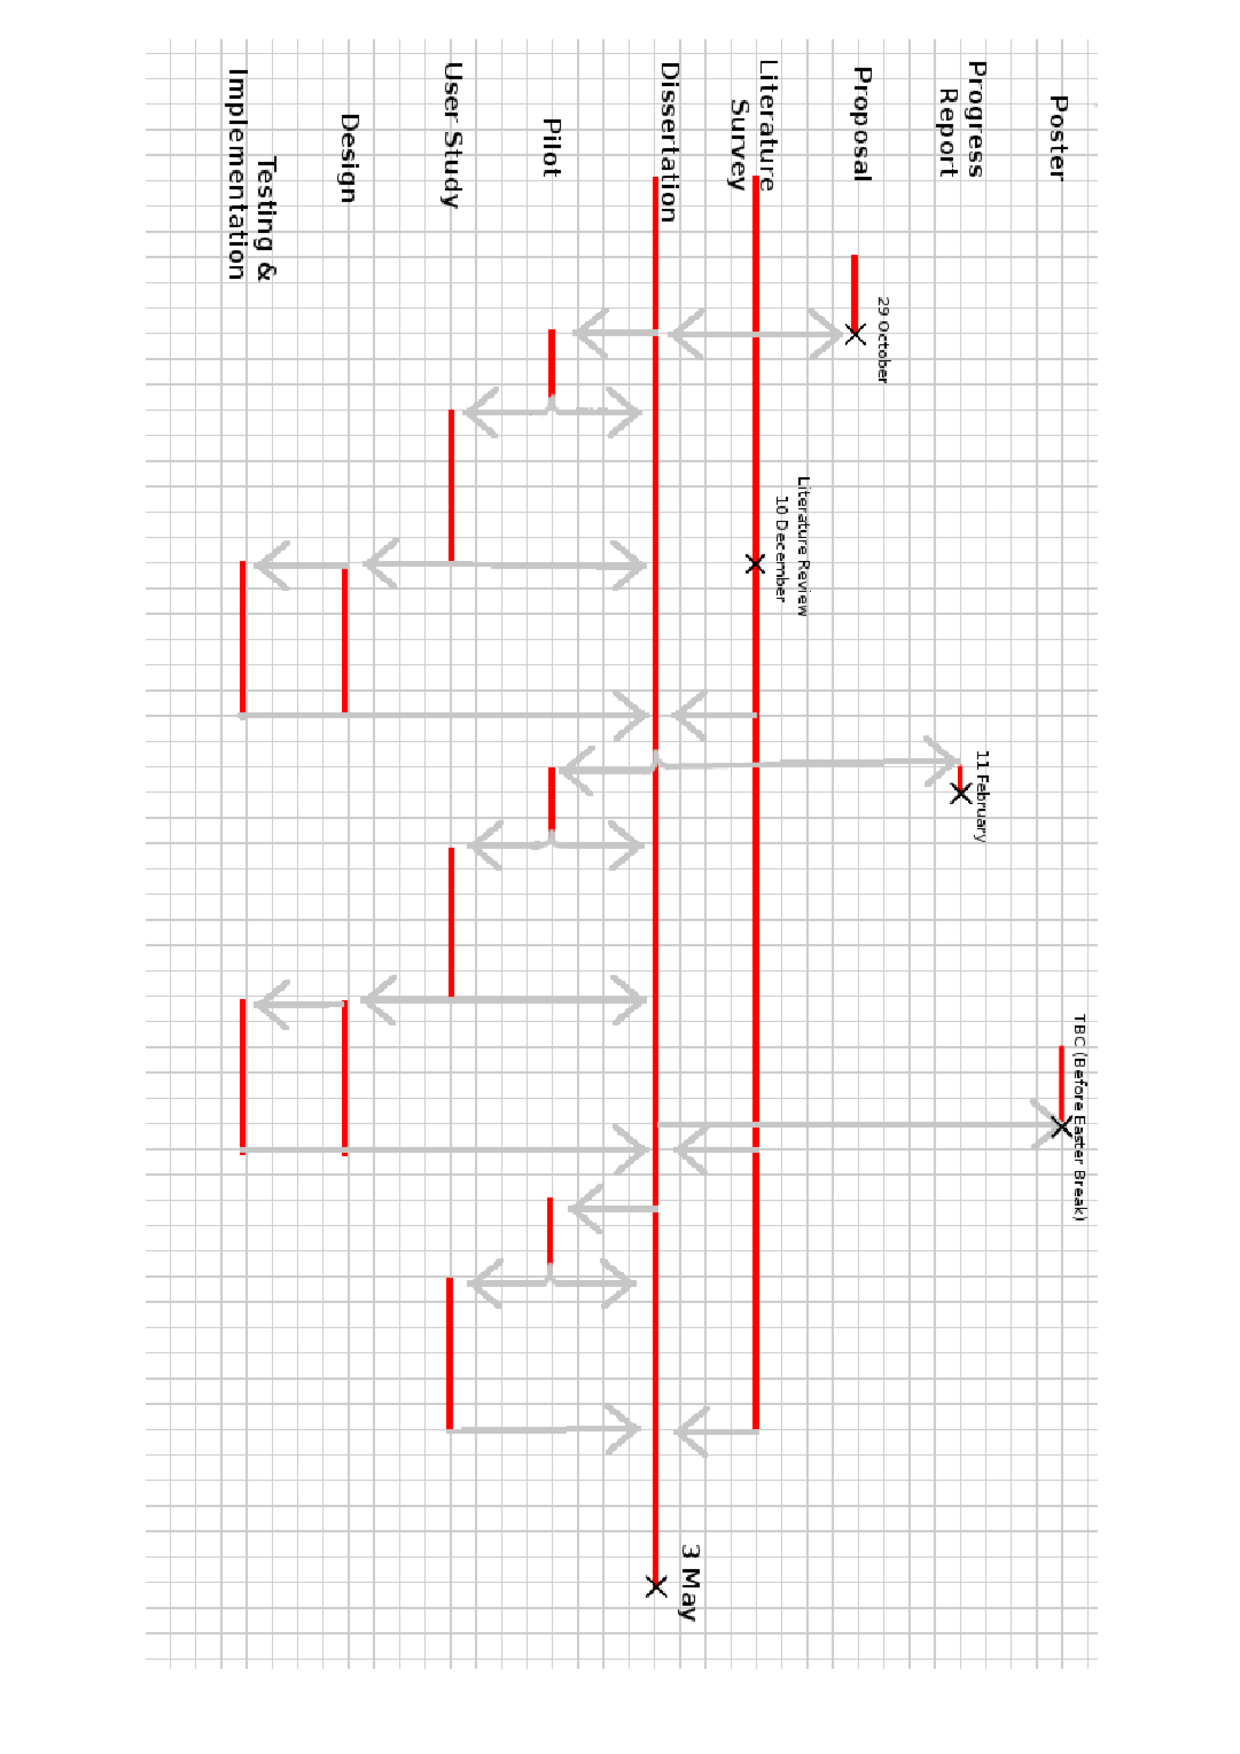
\includepdf[scale=0.7,pages=1,pagecommand=\subsection{Gantt
chart}\label{pdf:gantt}]{final_year_project-ganttchart.pdf}


\chapter{Required Resources}

I will now talk about the resources I require for the completion of this
dissertation, including the availability of these resources.

I will require users for my user study. These users must be proficient in at
least one programming language (declarative programming languages are niche in
and of themselves, never mind the discipline of programming, so some basic
knowledge is required in order to see useful patterns in User Interface Design).
Suitable candidates are First and Second Year
Computer Science students from most Universities in the UK. Their availability
is limited -- Christmas holidays and coursework deadlines may mean that certain
periods of the term are particularly busy for them. At Bath, suitable periods are
therefore November, January to Mid February (inclusive), Mid-March to April
(inclusive). It will be useful to procure free periods for other nearby
Universities to hedge my bets, and to have a decent random assignment of users so I
can make equivalent groups in my experiments.

The ACM Digital library, accessible via the Bath portal either from University
or from home via Single-sign-on is a valuable resource for research papers,
articles and references. The Cited-By feature will allow me to assert the
popularity/ranking of each resource. Another valuable resource is the Psychology
of Programming Interest Group, a ``[group of] people from diverse communities to explore
common interests in the psychological aspects of programming and in the
computational aspects of psychology'', with peer reviewed papers on particularly
relevant topics to my area of research.

I will require regular access to the Internet, Emacs with haskell-mode installed and Elm version 0.10
\cite{Elm2013a}. I will also need git for software source control, and
bitbucket.org for online, private backups of my work.
I require LaTeX to type up my dissertation, and have chosen texlive on Ubuntu 12.04.3
as my development environment of choice. The full development environment is
installed at the house I am staying in, in Bath, on my laptop. I am also able to
replicate this environment to a satisfactory level at Bath University on any
computer with access via Putty/SSH or similar to LCPU, as all the above software
can be installed and run on my Bath University account.

I am using Chromium Version 28.0.1500.71 Ubuntu 12.04
(28.0.1500.71-0ubuntu1.12.04.1) to run the Elm IDE, which is an important
dependency that may cause problems in getting Users in User Studies to run a
functionally equivalent browser. Only recent editions of Chrome, Chromium,
Firefox, Opera and Safari (not Internet Explorer) support Elm web programs.

\chapter{Ethical considerations}

In conducting User Studies, I will be interacting with people and collecting
data from them, so I must be considerate and mindful of those I talk to and the
information I handle.

An Ethical Checklist such as the one Bath University uses as it's template
\cite{Bath2013a} may assist my research such that I treat each participant
with care and respect. I may learn from the discoveries made by others -- in my
reading, I came across a paper (also mentioned earlier) that highlighted concerns that
participants under study had, and the paper detailed ways to mitigate these
concerns so as to make the participant feel that are informed and safe
\cite{Yates2012a}.

\bibliography{diss}
\addcontentsline{toc}{chapter}{Bibliography}

\printglossary
\addcontentsline{toc}{chapter}{Glossary}

\end{document}
